\documentclass{article}
\usepackage[utf8]{inputenc}
\usepackage{graphicx}
\usepackage{amsmath}
\graphicspath{ {./images/} }

\title{Bezier regression model}
\author{Jakob Drusany}
\date{November 2019}

\begin{document}

\maketitle

\section{Inspiration}
The bezier curve is calculated by providing $N$ points. The algorithm calculates the points by changing $t$ from 0 to 1. We can treat this model as kind a bijection. If we want to fit a bezier curve to a function, we can treat this model similarly to a neural network. We can then calculate an approximation using gradient descend.

\section{Forward propagation}
Here we have an example model at $N = 4$

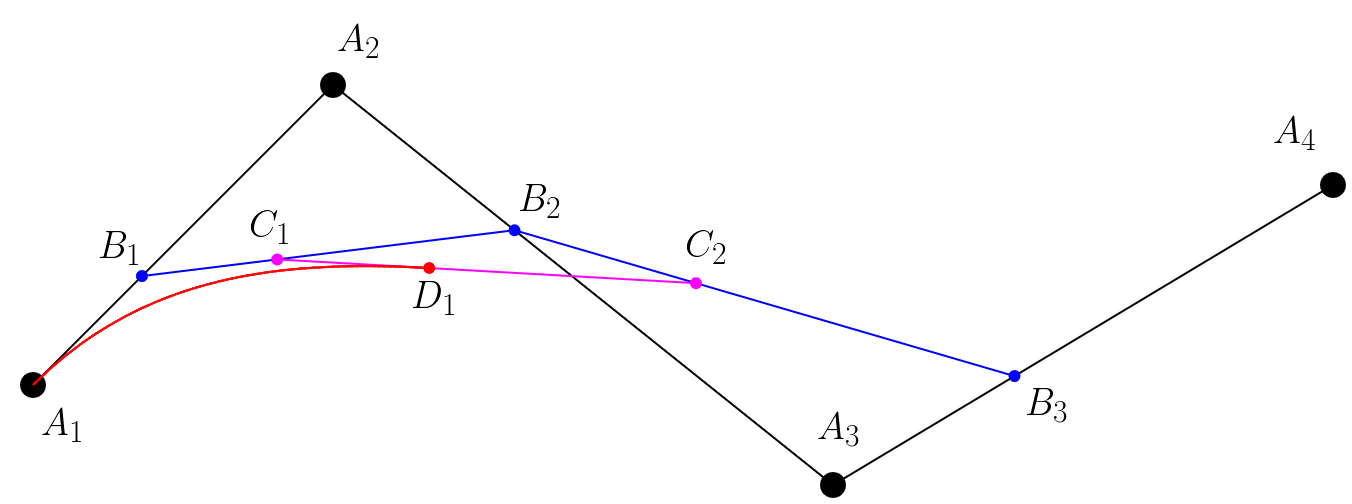
\includegraphics[width=\textwidth]{bezier}

First we have the "forward propagation" - calculating the $D_1$
\begin{equation} \label{eq:1}
    \vec{D_{n, t}} = P_t(\vec{C_{n, t}}, \vec{C_{n+1, t}})  
\end{equation}

\begin{equation} \label{eq:2}
    \vec{C_{m, t}} = P_t(\vec{B_{m, t}}, \vec{B_{m+1, t}})  
\end{equation}

\begin{equation} \label{eq:3}
    \vec{B_{k, t}} = P_t(\vec{A_{k, t}}, \vec{A_{k+1, t}})  
\end{equation}
\newpage
The function $P$ takes in 2 vectors and returns a single one. This returns the "midpoint" between the 2 points, with a given coefficient:
\begin{center}
    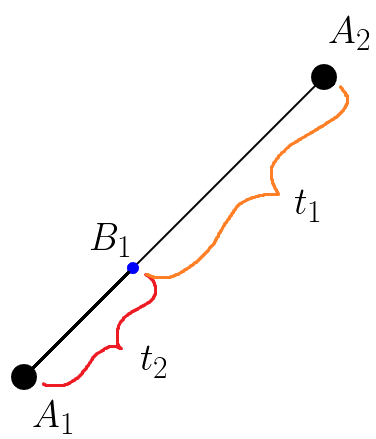
\includegraphics[scale=0.3]{t_ratio}
\end{center}
Where $t = \frac{t_2}{t_1}$, therefore:
\begin{equation}
    P_t(\vec{A_1}, \vec{A_2}) =  \vec{A_1} + (\vec{A_2} - \vec{A_1}) * t
\end{equation}
\section{Backpropagation}
To fit our bezier curve to a function $f(x)$, we have to calculate an error at each step. Using the mean square error, we can do this by the next equation (here $n$ is determined by how accurate we want our function to be):
\begin{equation} \label{eq:5}
    E = \sum_{t=0}^1\frac{1}{2}(f(x) - D_{1,t})^2
\end{equation}
The $x$ here is calculated by the same function $P$ using the first and the last point and the taking the x component.
If we want to minimize this error, we can calculate the derivatives with respect to the input points ($A_1, A_2, ..., A_n$), and then "go down the hill" with gradient descend. We have to approximate the y components of the vectors, so I will not be using vector notation from here forward. We can do this by applying the chain rule at each layer:
\begin{equation}
    \frac{\partial E}{\partial A_n} = \sum_{t=0}^1\sum_{n=1}^1\sum_{m=1}^2\sum_{k=1}^3 \frac{\partial E}{\partial D_{1, t}}*\frac{\partial D_{1, t}}{\partial C_{m, t}}*\frac{\partial C_{m, t}}{\partial B_{k, t}}*\frac{\partial B_{k, t}}{\partial A_{i, t}}
\end{equation}
First lets define the derivatives of our function $P$
\begin{equation} \label{eq:7}
    \frac{\partial P_t(A_1, A_2)}{\partial A_1} = \frac{\partial \left[A_1 + (A_2 - A_1) * t\right]}{\partial A_1} = 1 - t
\end{equation}
\begin{equation}
    \frac{\partial P_t(A_1, A_2)}{\partial A_2} = \frac{\partial \left[A_1 + (A_2 - A_1) * t\right]}{\partial A_2} = t
\end{equation}

The first factor in the chain rule is the derivative of (\ref{eq:5}):
\begin{equation}
    \frac{\partial E}{\partial D_{1, t}} = \frac{\partial}{\partial D_{1, t}}\left[\sum_{t_1=0}^1\frac{1}{2}(f(x) - D_{1,t_1})^2\right] = (D_{t,1} - f(x))
\end{equation}
The second factor in the chain rule is the derivative of (\ref{eq:1}):
Here there is a difference in the derivative with respect to $ C_m $, if it is the first argument of the function, we use (\ref{eq:7}), else we use (\ref{eq:8})
\begin{equation}
    \frac{\partial D_{1, t}}{\partial C_{m, t}} = \frac{\partial \left[P_t(C_{n, t}, C_{n+1, t})\right]}{\partial C_{m, t}} = \begin{cases} 
      1 - t & m = n \\
      t & m = n+1
   \end{cases}
\end{equation}
All other factors are computed the same.
General formula where $ K_{t} $ is the one layer forward of $J_{m,t}$ and isn't the last layer.
\begin{equation}
	\frac{\partial K_{t}}{\partial J_{n,t}} = \frac{\partial \left[P_t(J_{n, t}, J_{n+1, t})\right]}{\partial J_{n, t}} + \frac{\partial \left[P_t(J_{n-1, t}, J_{n, t})\right]}{\partial J_{n, t}}
\end{equation}

\end{document}
